\documentclass[12pt]{report}
\usepackage{amssymb}
\usepackage{multicol}
\usepackage{graphicx}
\usepackage{subfigure}
\usepackage{verbatim}
\usepackage[letterpaper,left=1cm,right=2cm, top=1.5cm,
bottom=1.5cm,head=0cm,foot=1cm]{geometry}

\parindent=0in


\newcommand{\m}{\mbox{ m }}
\newcommand{\kg}{\mbox{ kg }}
\newcommand{\s}{\mbox{ s }}
\newcommand{\ke}{\mbox{\small KE}}
\newcommand{\pe}{\mbox{\small PE}}


\newcommand{ \probDir}[1]{{ \bf\small #1 \mbox{  }}}

\newcommand{ \breakList}{\setcounter{saveenum}{\value{enumi}} \end{enumerate}}
\newcommand{ \contList}{\begin{enumerate} \setcounter{enumi}{\value{saveenum}}}

\newcounter{saveenum}

\def \wspace{5cm}

%%%%%%%%%%%%%%%%%%%%%%%%%%%%%%%%%%%%%%%%%
\begin{document}

{\bf{Honors Physics} \hfill {Review Party} \hfill {Mr. Kelley}} \\ \\
%%%%%%%%%%
$\rho=mv$ \hfill $\ke=\frac{1}{2}mv^2$ \hfill $\pe=mgh$ \hfill $\rho_\circ = \rho_f$ \hfill $\ke_\circ + \pe_\circ = \ke_f + \pe_f$


\begin{enumerate}
\item $m_1 = 3 \kg$ smacks into the stationary $m_2 = 5\kg$ at 20 m/s.  If $m_1$ bounces back at 6 m/s, what is the final velocity of $m_2$?  What if $m_1$ comes to rest after hitting $m_2$? \\ \vspace{1cm}

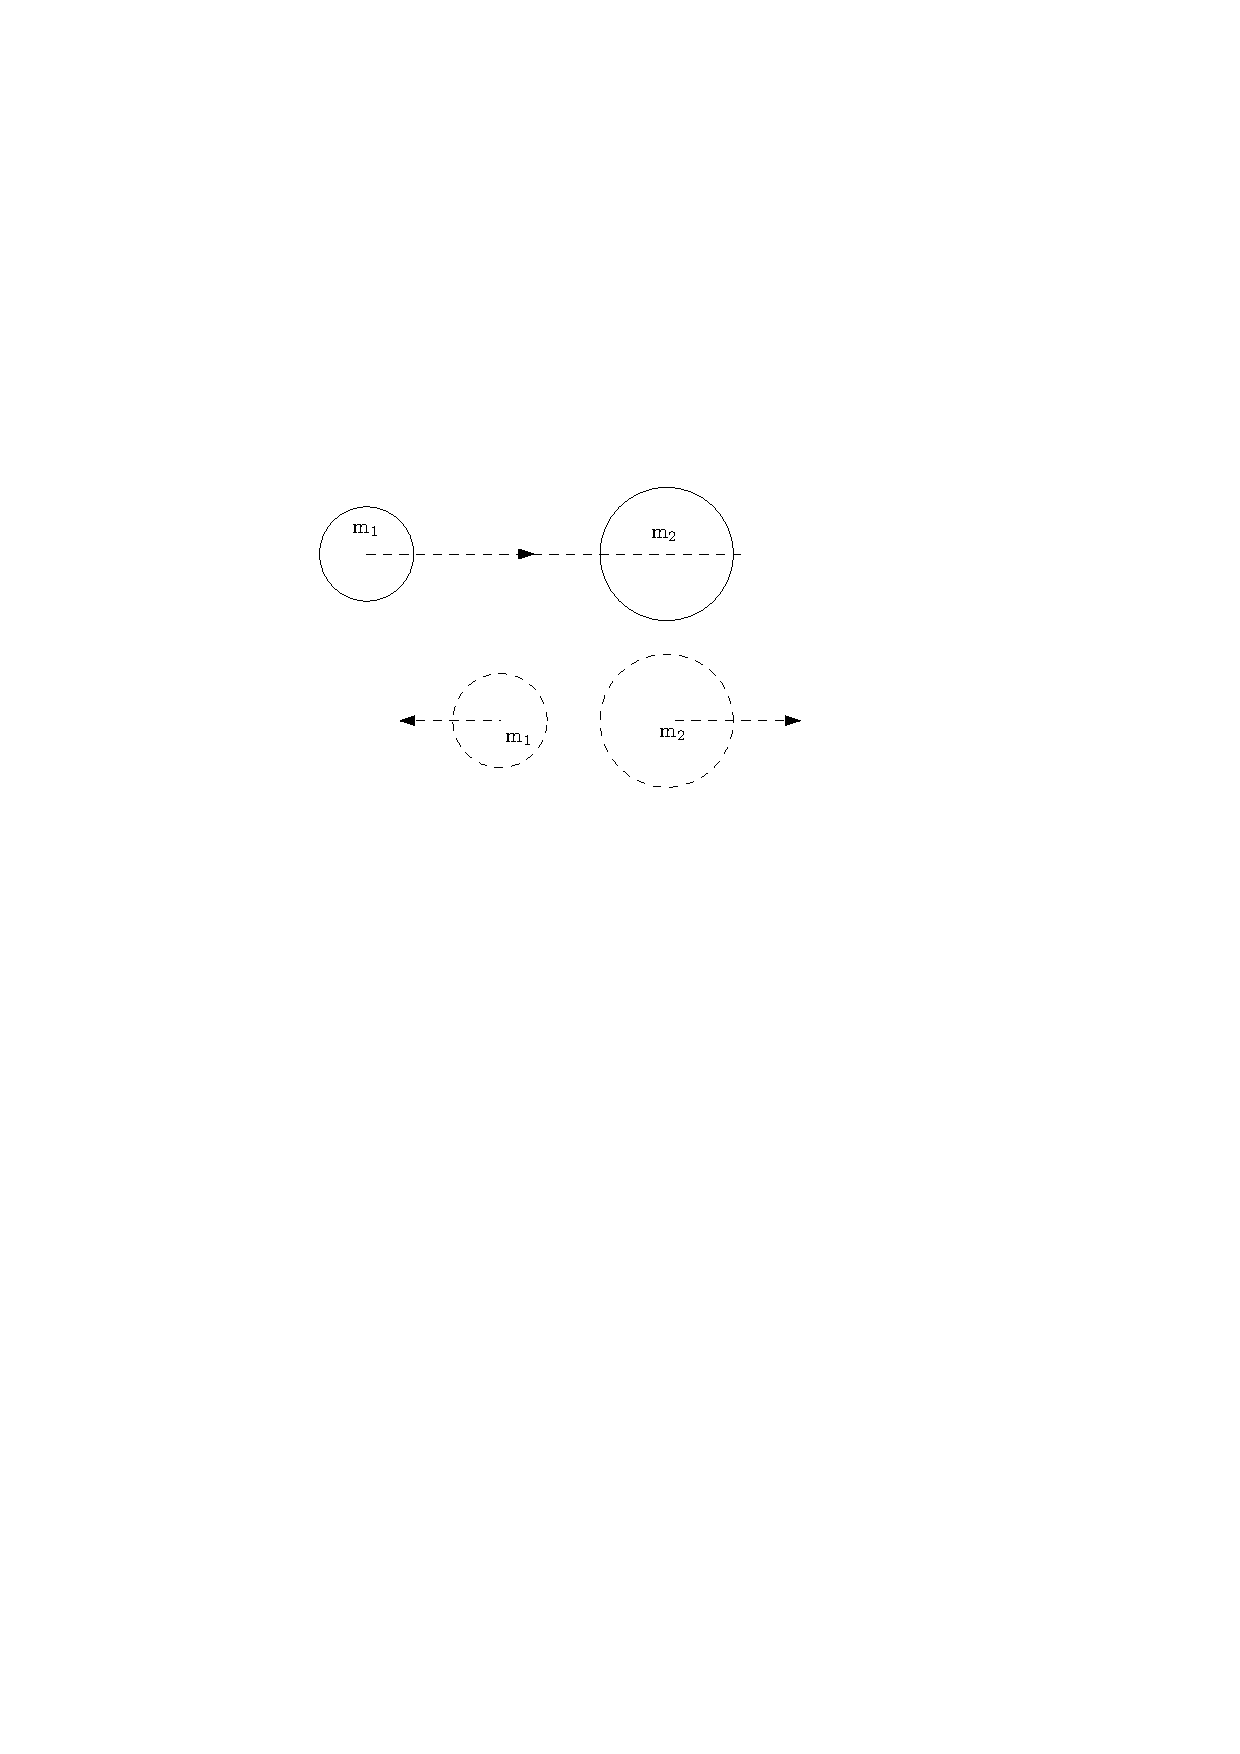
\includegraphics[scale = 1]{1dCollision_bounceBack}
\vspace{.75cm}

\item $m_1 = 5 \kg$ is traveling at 10 m/s and collides with $m_2 = 5 \kg$ which is at rest.  They stick together.  How fast are they moving? \\ \vspace{1cm}

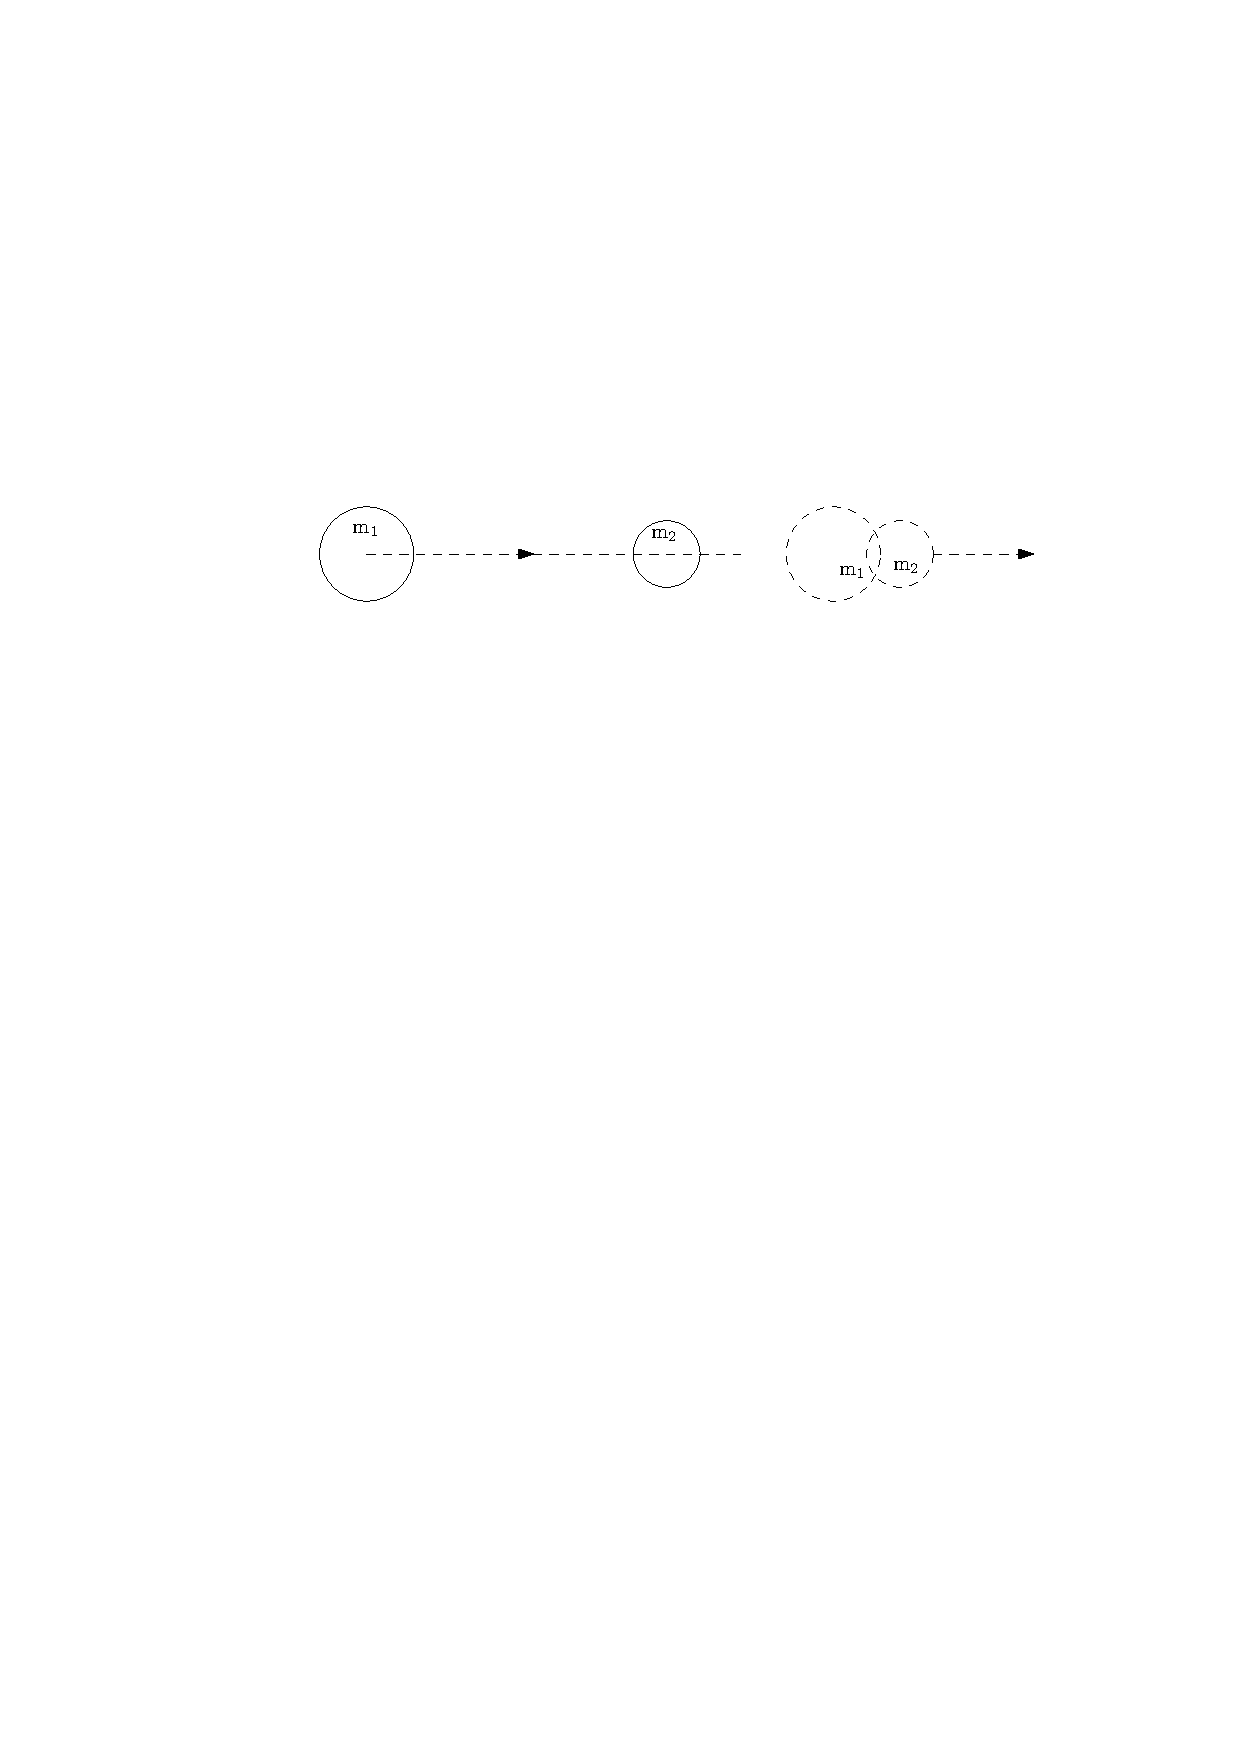
\includegraphics[scale = 1]{1dCollision_stick}
\vspace{.75cm}

\item $m_1 = 1 \kg$ collides with $m_2 = 2 \kg$, head-on.  They were both initially traveling at 7 m/s.  If $m_2$ recoils with a speed of 2 m/s, how fast and in what direction is $m_1$ going after the collision? \\ \vspace{1cm}

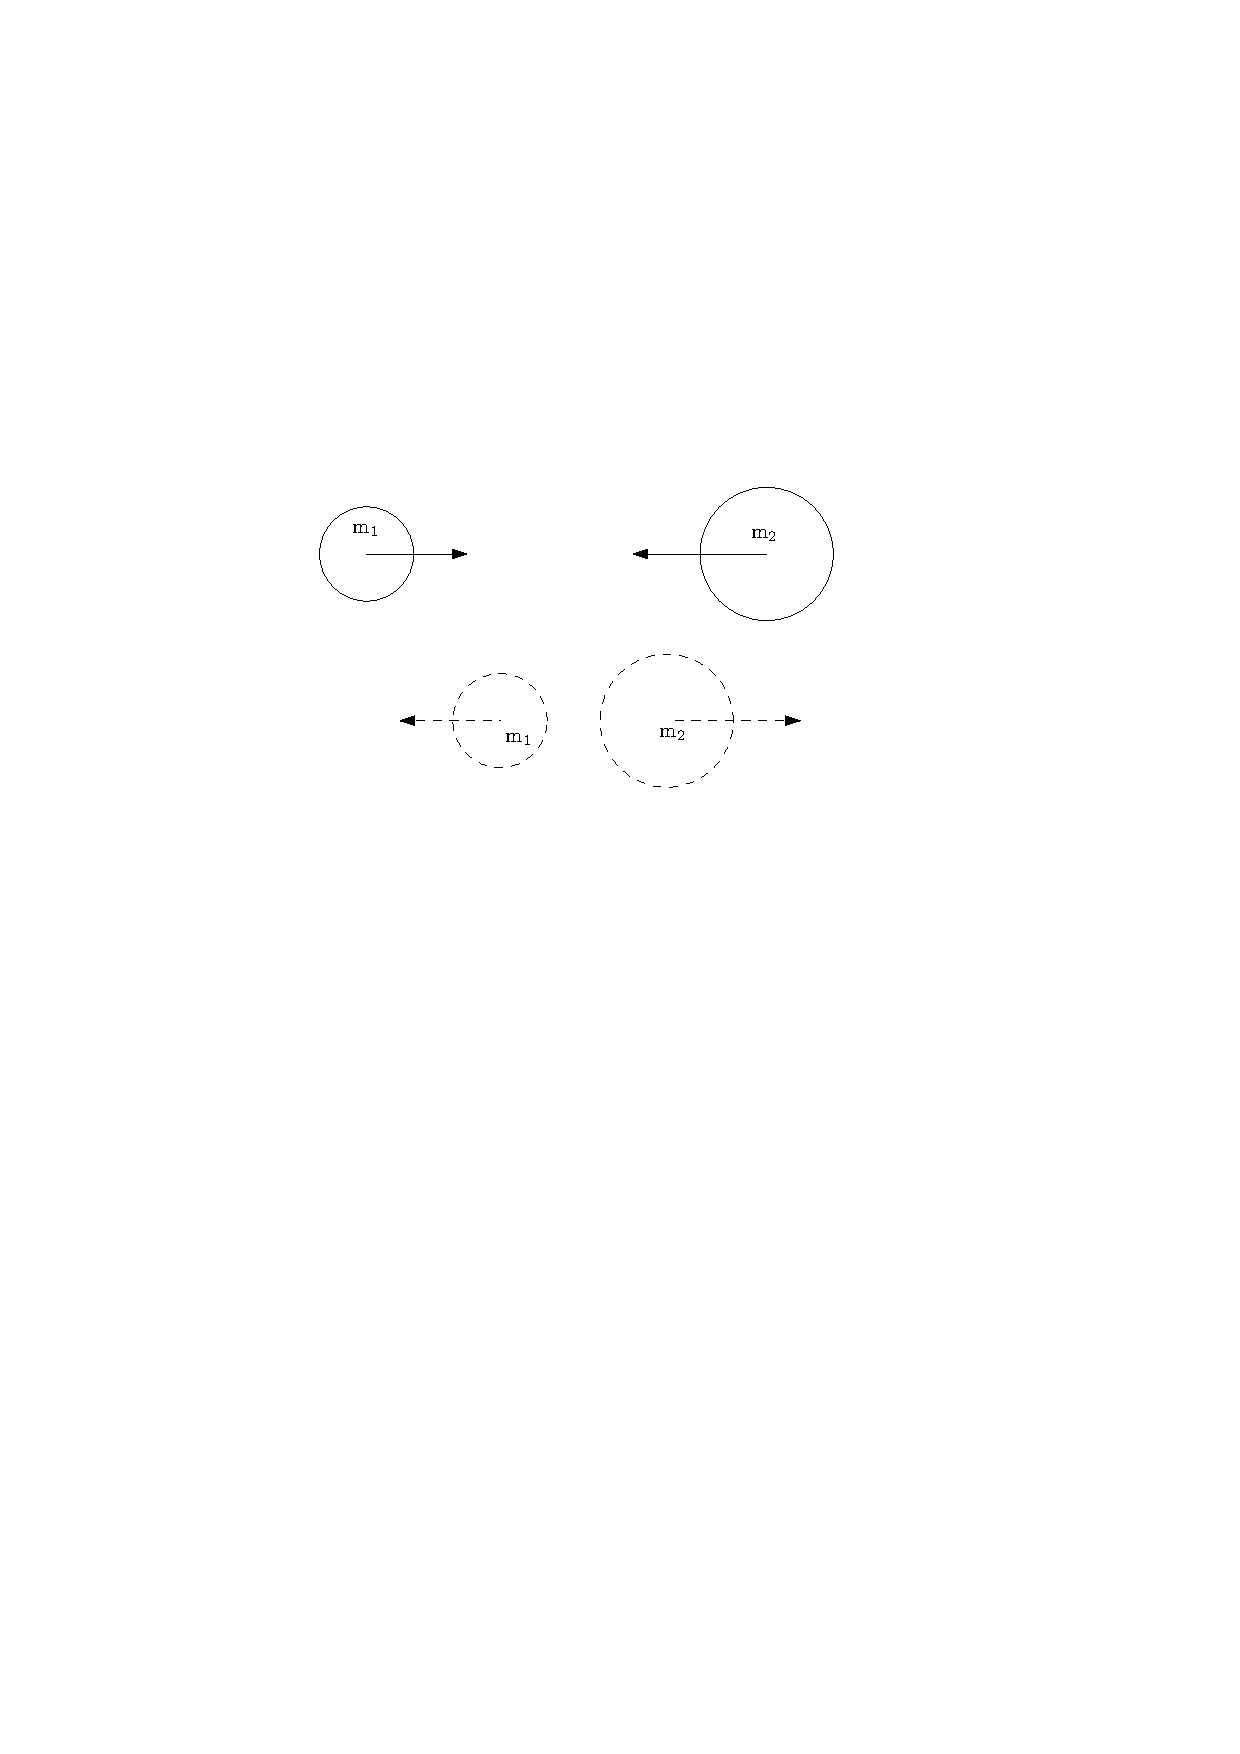
\includegraphics[scale = 1]{1dCollision_headOn}
\vspace{.75cm}

\item $m_1 = 3 \kg$ collides with $m_2 = 2 \kg$, sending $m_2$ off at an angle of $25^\circ$ with a speed of 5 m/s.  If $m_1$ was initially traveling at 4 m/s, and $m_2$ was initially at rest, how fast and at what angle is $m_1$ going now? \\ \vspace{1cm}

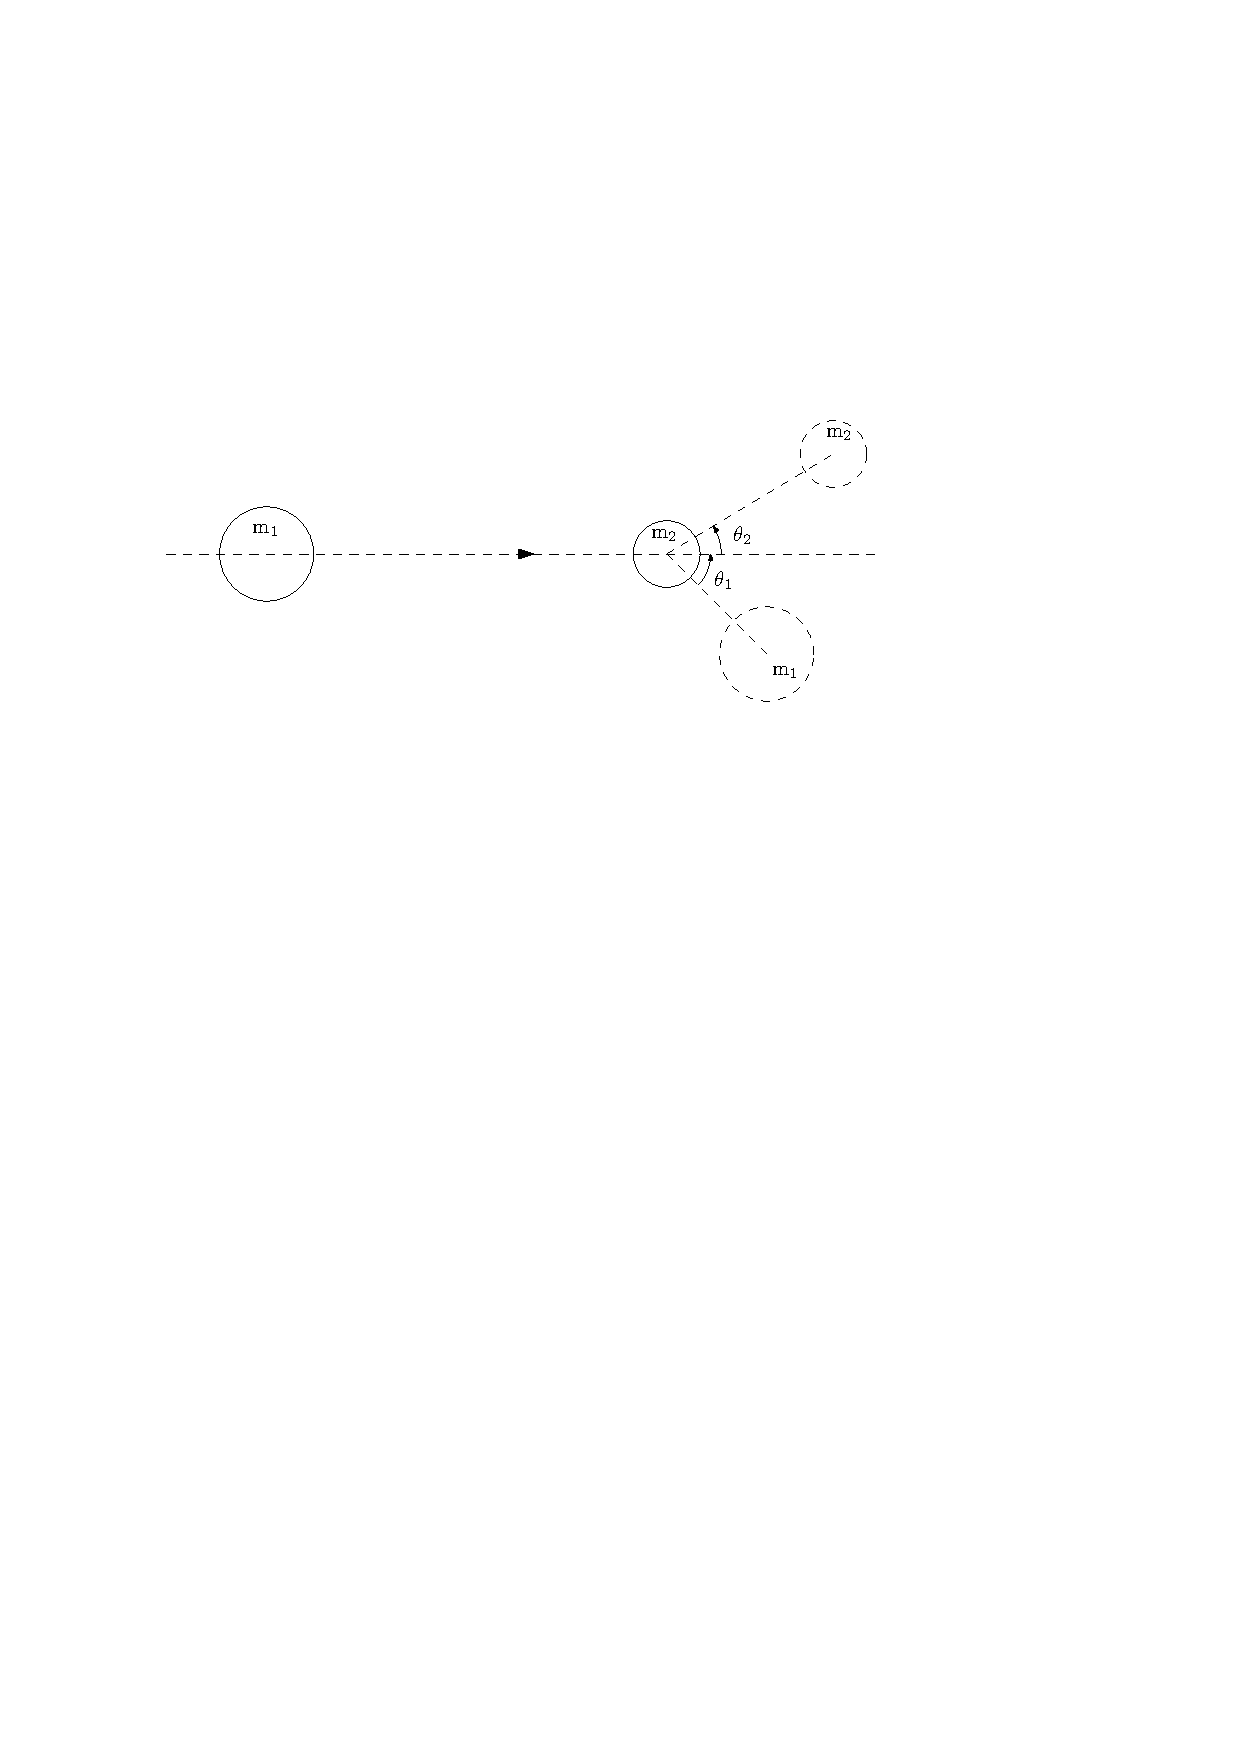
\includegraphics[scale = 1]{2dCollision_1}
\vspace{.75cm}

\item For the following picture, what is $v_1, v_2, v_3,$ and $v_4$? (This is a ball rolling on a track, and there is no friction)  \\ \vspace{1cm}

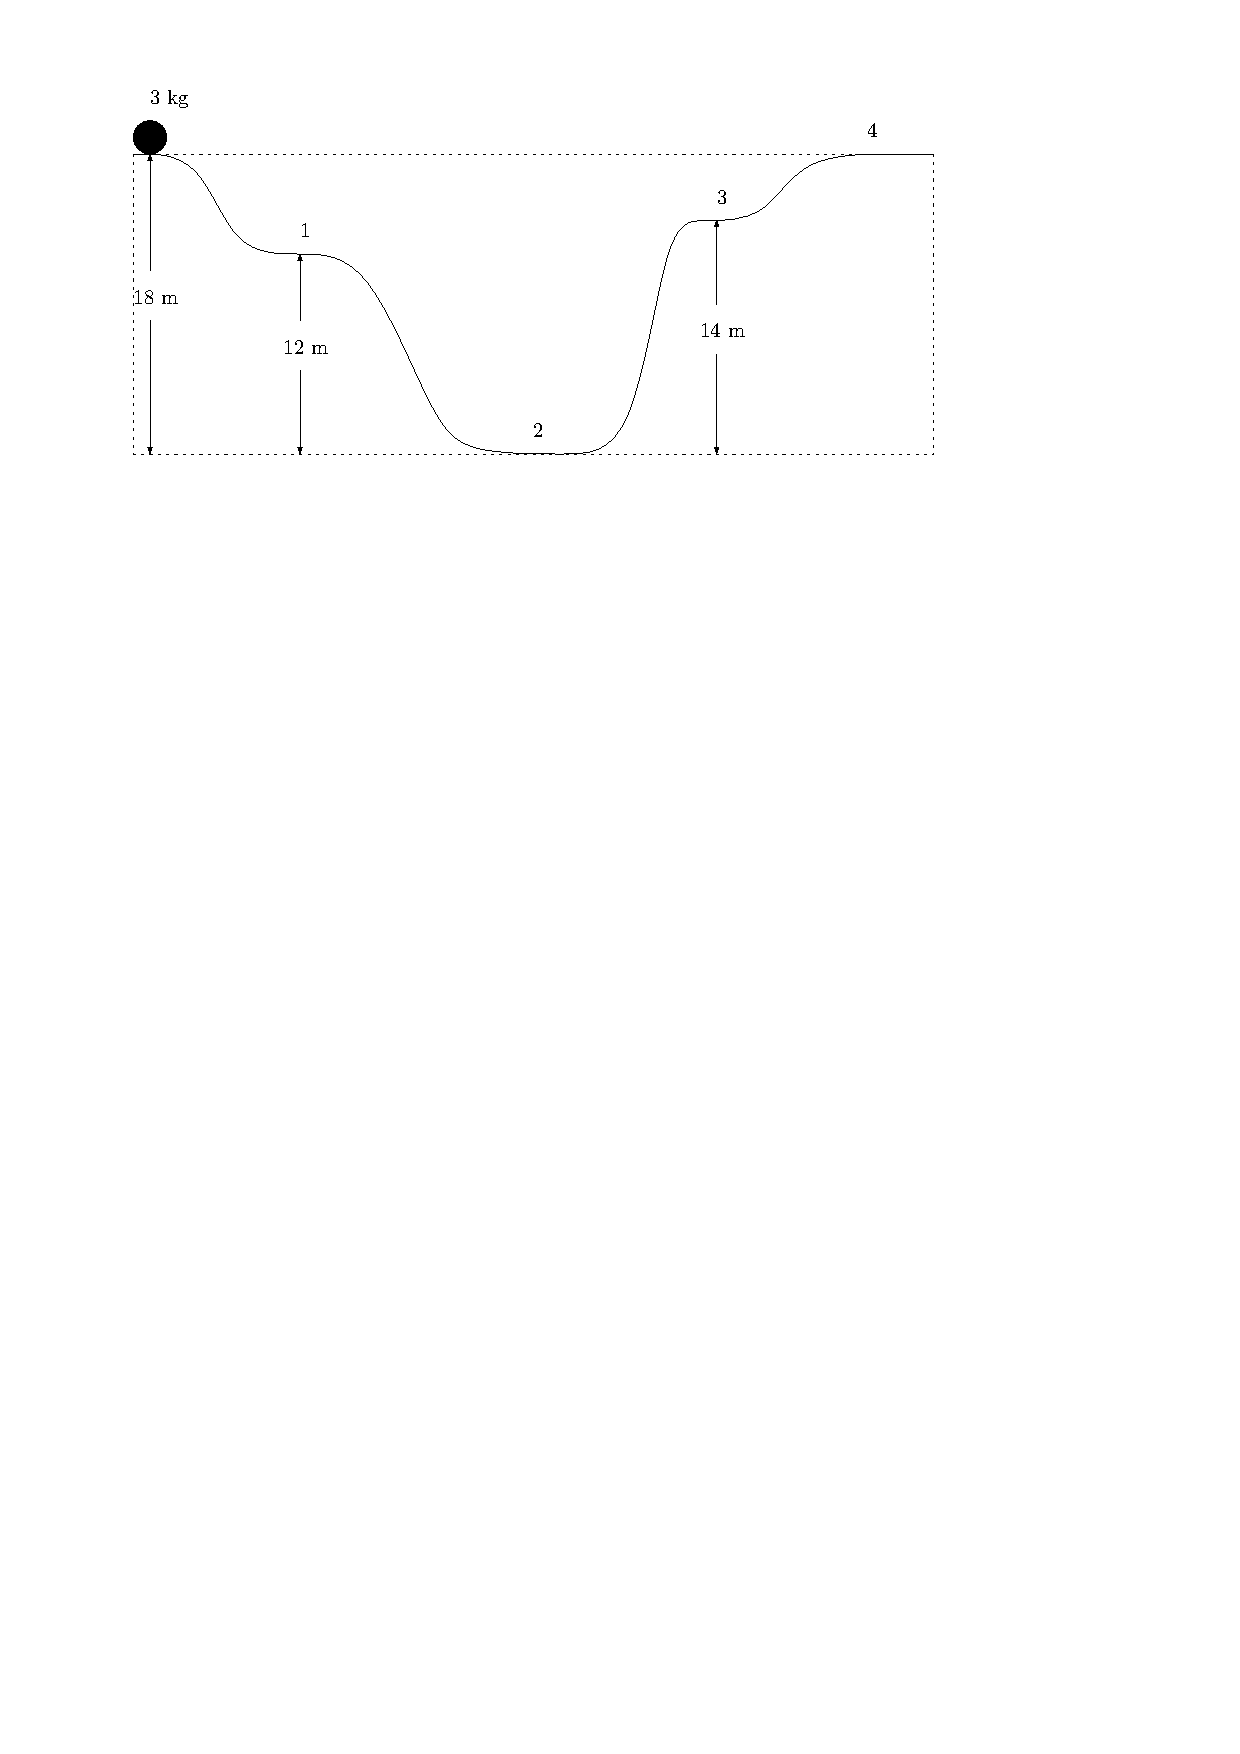
\includegraphics[scale = 1]{energyCoaster}
\vspace{.75cm}


\end{enumerate}




\end{document}